\begin{pastexam}[label={px:ncku-108-prog-08}]{成大資訊聯招 108 學年度 第 8 題}
（追蹤）

(10\%) Write the breadth first spanning tree starting at node 0 (visit the smaller number first).
\begin{center}
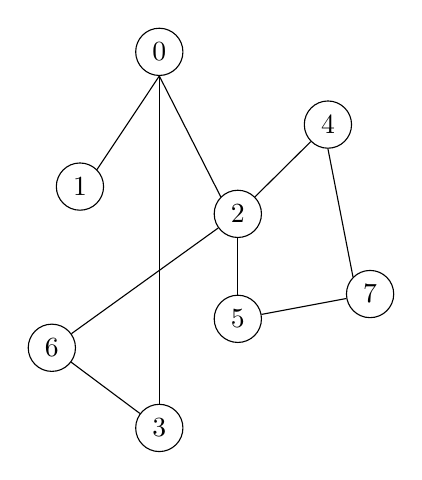
\begin{tikzpicture}[x=0.0105cm,y=-0.0105cm,
  v/.style={circle,draw,inner sep=0pt,minimum size=6mm}]
\node[v] (0) at (228,72) {0};
\node[v] (1) at (132,235) {1};
\node[v] (2) at (323,268) {2};
\node[v] (4) at (432,160) {4};
\node[v] (5) at (323,395) {5};
\node[v] (7) at (483,365) {7};
\node[v] (6) at (98,430) {6};
\node[v] (3) at (228,527) {3};
\draw (0.south) -- (1.north east);
\draw (0.south) -- (3.north);
\draw (0.south) -- (2.north west);
\draw (4) -- (2) (2) -- (6);
\draw (2) -- (5);
\draw (5) -- (7);
\draw (4.south) -- (7.north west);
\draw (6) -- (3);
\end{tikzpicture}
\end{center}
\end{pastexam}

\begin{pastsoln}
答案：BFS 生成樹的邊是 $(0,1)$、$(0,2)$、$(0,3)$、$(2,4)$、$(2,5)$、$(2,6)$、$(4,7)$；造訪順序
$0, 1, 2, 3, 4, 5, 6, 7$。

圖上的邊共 $9$ 條：$\{0,1\}$、$\{0,2\}$、$\{0,3\}$、$\{2,4\}$、$\{2,5\}$、$\{2,6\}$、$\{3,6\}$、$\{4,7\}$、$\{5,7\}$
（從 $4$ 往左下的線經過 $2$ 再到 $6$，是 $\{2,4\}$、$\{2,6\}$ 兩條邊；從 $0$ 垂直往下的線一路到 $3$，中間不碰其他頂點）。
鄰接串列依編號由小到大排：
\begin{center}
\small
\begin{tabular}{c*{8}{c}}
\toprule
頂點 & 0 & 1 & 2 & 3 & 4 & 5 & 6 & 7 \\
\midrule
鄰居 & 1, 2, 3 & 0 & 0, 4, 5, 6 & 0, 6 & 2, 7 & 2, 7 & 2, 3 & 4, 5 \\
\bottomrule
\end{tabular}
\end{center}

照資結書虛擬碼~21.1 追蹤：取出佇列最前面的頂點，依序看它的鄰居，還沒發現的就標記、記下樹邊、放進佇列尾端。
\begin{center}
\small
\begin{tabular}{clll}
\toprule
取出 & 掃描鄰居 & 新的樹邊 & 之後的佇列 \\
\midrule
（開始） & & & $\langle 0 \rangle$ \\
$0$ & $1, 2, 3$ 都是新的 & $(0,1)$、$(0,2)$、$(0,3)$ & $\langle 1, 2, 3 \rangle$ \\
$1$ & $0$ 已發現 & & $\langle 2, 3 \rangle$ \\
$2$ & $0$ 已發現；$4, 5, 6$ 是新的 & $(2,4)$、$(2,5)$、$(2,6)$ & $\langle 3, 4, 5, 6 \rangle$ \\
$3$ & $0$、$6$ 都已發現 & & $\langle 4, 5, 6 \rangle$ \\
$4$ & $2$ 已發現；$7$ 是新的 & $(4,7)$ & $\langle 5, 6, 7 \rangle$ \\
$5$ & $2$、$7$ 都已發現 & & $\langle 6, 7 \rangle$ \\
$6$ & $2$、$3$ 都已發現 & & $\langle 7 \rangle$ \\
$7$ & $4$、$5$ 都已發現 & & $\langle\,\rangle$ \\
\bottomrule
\end{tabular}
\end{center}

$8$ 個頂點、$7$ 條樹邊。 沒用到的兩條邊是 $\{3,6\}$ 和 $\{5,7\}$：掃到它們時另一端已經發現了。 注意 $6$ 是由 $2$
發現的，不是 $3$，因為 $2$ 比 $3$ 先出佇列；$7$ 由 $4$ 發現，因為 $4$ 比 $5$ 先出佇列。

\begin{center}
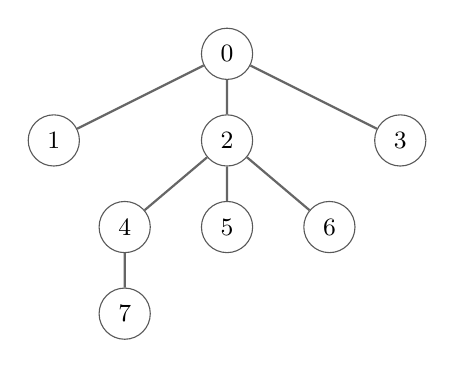
\begin{tikzpicture}[
    btn/.style={circle, draw=black!65, line width=0.4pt, minimum size=6.5mm, inner sep=0pt, font=\small},
    level distance=11mm, edge from parent/.style={draw=black!60, thick},
    level 1/.style={sibling distance=22mm}, level 2/.style={sibling distance=13mm}]
\node[btn] {0}
    child {node[btn] {1}}
    child {node[btn] {2}
        child {node[btn] {4} child {node[btn] {7}}}
        child {node[btn] {5}}
        child {node[btn] {6}}}
    child {node[btn] {3}};
\end{tikzpicture}
\end{center}
樹上每個頂點的深度就是它到 $0$ 的最短距離（邊數）：$1, 2, 3$ 是 $1$，$4, 5, 6$ 是 $2$，$7$ 是 $3$。
\end{pastsoln}
